% Created by tikzDevice version 0.10.1 on 2016-12-25 11:11:45
% !TEX encoding = UTF-8 Unicode
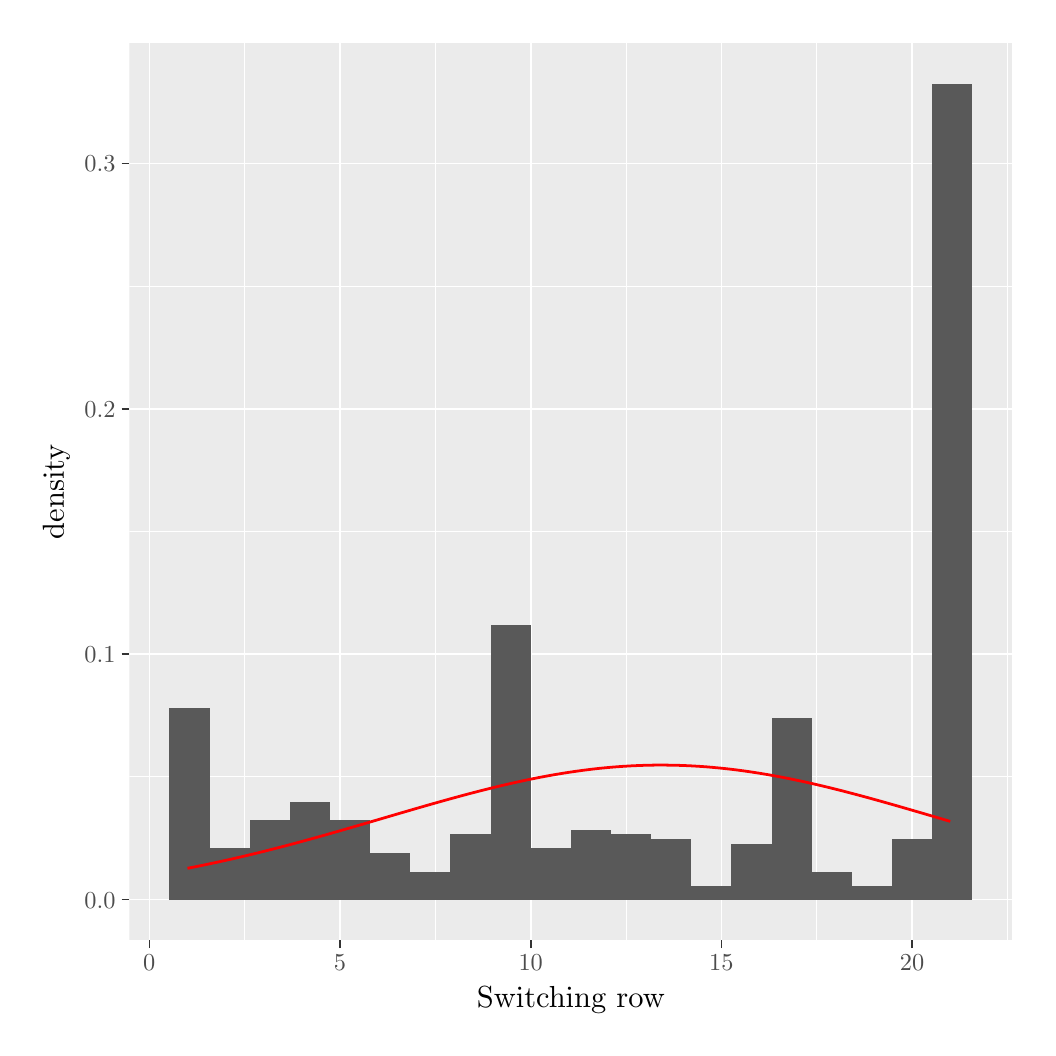
\begin{tikzpicture}[x=1pt,y=1pt]
\definecolor{fillColor}{RGB}{255,255,255}
\path[use as bounding box,fill=fillColor,fill opacity=0.00] (0,0) rectangle (361.35,361.35);
\begin{scope}
\path[clip] (  0.00,  0.00) rectangle (361.35,361.35);
\definecolor{drawColor}{RGB}{255,255,255}
\definecolor{fillColor}{RGB}{255,255,255}

\path[draw=drawColor,line width= 0.6pt,line join=round,line cap=round,fill=fillColor] (  0.00,  0.00) rectangle (361.35,361.35);
\end{scope}
\begin{scope}
\path[clip] ( 36.71, 31.53) rectangle (355.85,355.85);
\definecolor{fillColor}{gray}{0.92}

\path[fill=fillColor] ( 36.71, 31.53) rectangle (355.85,355.85);
\definecolor{drawColor}{RGB}{255,255,255}

\path[draw=drawColor,line width= 0.3pt,line join=round] ( 36.71, 90.61) --
	(355.85, 90.61);

\path[draw=drawColor,line width= 0.3pt,line join=round] ( 36.71,179.28) --
	(355.85,179.28);

\path[draw=drawColor,line width= 0.3pt,line join=round] ( 36.71,267.95) --
	(355.85,267.95);

\path[draw=drawColor,line width= 0.3pt,line join=round] ( 78.42, 31.53) --
	( 78.42,355.85);

\path[draw=drawColor,line width= 0.3pt,line join=round] (147.32, 31.53) --
	(147.32,355.85);

\path[draw=drawColor,line width= 0.3pt,line join=round] (216.23, 31.53) --
	(216.23,355.85);

\path[draw=drawColor,line width= 0.3pt,line join=round] (285.13, 31.53) --
	(285.13,355.85);

\path[draw=drawColor,line width= 0.3pt,line join=round] (354.04, 31.53) --
	(354.04,355.85);

\path[draw=drawColor,line width= 0.6pt,line join=round] ( 36.71, 46.27) --
	(355.85, 46.27);

\path[draw=drawColor,line width= 0.6pt,line join=round] ( 36.71,134.94) --
	(355.85,134.94);

\path[draw=drawColor,line width= 0.6pt,line join=round] ( 36.71,223.62) --
	(355.85,223.62);

\path[draw=drawColor,line width= 0.6pt,line join=round] ( 36.71,312.29) --
	(355.85,312.29);

\path[draw=drawColor,line width= 0.6pt,line join=round] ( 43.96, 31.53) --
	( 43.96,355.85);

\path[draw=drawColor,line width= 0.6pt,line join=round] (112.87, 31.53) --
	(112.87,355.85);

\path[draw=drawColor,line width= 0.6pt,line join=round] (181.77, 31.53) --
	(181.77,355.85);

\path[draw=drawColor,line width= 0.6pt,line join=round] (250.68, 31.53) --
	(250.68,355.85);

\path[draw=drawColor,line width= 0.6pt,line join=round] (319.58, 31.53) --
	(319.58,355.85);
\definecolor{fillColor}{gray}{0.35}

\path[fill=fillColor] ( 51.22, 46.27) rectangle ( 65.72,115.35);

\path[fill=fillColor] ( 65.72, 46.27) rectangle ( 80.23, 64.81);

\path[fill=fillColor] ( 80.23, 46.27) rectangle ( 94.74, 74.91);

\path[fill=fillColor] ( 94.74, 46.27) rectangle (109.24, 81.65);

\path[fill=fillColor] (109.24, 46.27) rectangle (123.75, 74.91);

\path[fill=fillColor] (123.75, 46.27) rectangle (138.26, 63.12);

\path[fill=fillColor] (138.26, 46.27) rectangle (152.76, 56.38);

\path[fill=fillColor] (152.76, 46.27) rectangle (167.27, 69.86);

\path[fill=fillColor] (167.27, 46.27) rectangle (181.77,145.67);

\path[fill=fillColor] (181.77, 46.27) rectangle (196.28, 64.81);

\path[fill=fillColor] (196.28, 46.27) rectangle (210.79, 71.54);

\path[fill=fillColor] (210.79, 46.27) rectangle (225.29, 69.86);

\path[fill=fillColor] (225.29, 46.27) rectangle (239.80, 68.17);

\path[fill=fillColor] (239.80, 46.27) rectangle (254.31, 51.33);

\path[fill=fillColor] (254.31, 46.27) rectangle (268.81, 66.49);

\path[fill=fillColor] (268.81, 46.27) rectangle (283.32,111.98);

\path[fill=fillColor] (283.32, 46.27) rectangle (297.82, 56.38);

\path[fill=fillColor] (297.82, 46.27) rectangle (312.33, 51.33);

\path[fill=fillColor] (312.33, 46.27) rectangle (326.84, 68.17);

\path[fill=fillColor] (326.84, 46.27) rectangle (341.34,341.11);
\definecolor{drawColor}{RGB}{255,0,0}

\path[draw=drawColor,line width= 1.0pt,line join=round] ( 57.75, 57.59) --
	( 60.50, 58.13) --
	( 63.26, 58.69) --
	( 66.01, 59.26) --
	( 68.77, 59.85) --
	( 71.53, 60.45) --
	( 74.28, 61.07) --
	( 77.04, 61.71) --
	( 79.80, 62.36) --
	( 82.55, 63.02) --
	( 85.31, 63.70) --
	( 88.06, 64.40) --
	( 90.82, 65.10) --
	( 93.58, 65.82) --
	( 96.33, 66.55) --
	( 99.09, 67.30) --
	(101.84, 68.05) --
	(104.60, 68.81) --
	(107.36, 69.58) --
	(110.11, 70.37) --
	(112.87, 71.15) --
	(115.63, 71.95) --
	(118.38, 72.75) --
	(121.14, 73.55) --
	(123.89, 74.36) --
	(126.65, 75.17) --
	(129.41, 75.98) --
	(132.16, 76.79) --
	(134.92, 77.60) --
	(137.68, 78.40) --
	(140.43, 79.21) --
	(143.19, 80.00) --
	(145.94, 80.79) --
	(148.70, 81.57) --
	(151.46, 82.34) --
	(154.21, 83.10) --
	(156.97, 83.85) --
	(159.73, 84.59) --
	(162.48, 85.30) --
	(165.24, 86.01) --
	(167.99, 86.69) --
	(170.75, 87.36) --
	(173.51, 88.00) --
	(176.26, 88.62) --
	(179.02, 89.22) --
	(181.77, 89.80) --
	(184.53, 90.35) --
	(187.29, 90.87) --
	(190.04, 91.37) --
	(192.80, 91.83) --
	(195.56, 92.27) --
	(198.31, 92.67) --
	(201.07, 93.05) --
	(203.82, 93.39) --
	(206.58, 93.70) --
	(209.34, 93.97) --
	(212.09, 94.21) --
	(214.85, 94.41) --
	(217.61, 94.58) --
	(220.36, 94.71) --
	(223.12, 94.81) --
	(225.87, 94.87) --
	(228.63, 94.89) --
	(231.39, 94.87) --
	(234.14, 94.82) --
	(236.90, 94.74) --
	(239.65, 94.61) --
	(242.41, 94.45) --
	(245.17, 94.26) --
	(247.92, 94.02) --
	(250.68, 93.76) --
	(253.44, 93.46) --
	(256.19, 93.13) --
	(258.95, 92.76) --
	(261.70, 92.36) --
	(264.46, 91.93) --
	(267.22, 91.47) --
	(269.97, 90.98) --
	(272.73, 90.47) --
	(275.49, 89.92) --
	(278.24, 89.35) --
	(281.00, 88.76) --
	(283.75, 88.14) --
	(286.51, 87.50) --
	(289.27, 86.84) --
	(292.02, 86.16) --
	(294.78, 85.46) --
	(297.53, 84.74) --
	(300.29, 84.01) --
	(303.05, 83.27) --
	(305.80, 82.51) --
	(308.56, 81.74) --
	(311.32, 80.96) --
	(314.07, 80.18) --
	(316.83, 79.38) --
	(319.58, 78.58) --
	(322.34, 77.78) --
	(325.10, 76.97) --
	(327.85, 76.16) --
	(330.61, 75.35) --
	(333.37, 74.54);
\end{scope}
\begin{scope}
\path[clip] (  0.00,  0.00) rectangle (361.35,361.35);
\definecolor{drawColor}{gray}{0.30}

\node[text=drawColor,anchor=base east,inner sep=0pt, outer sep=0pt, scale=  0.88] at ( 31.76, 43.24) {0.0};

\node[text=drawColor,anchor=base east,inner sep=0pt, outer sep=0pt, scale=  0.88] at ( 31.76,131.91) {0.1};

\node[text=drawColor,anchor=base east,inner sep=0pt, outer sep=0pt, scale=  0.88] at ( 31.76,220.59) {0.2};

\node[text=drawColor,anchor=base east,inner sep=0pt, outer sep=0pt, scale=  0.88] at ( 31.76,309.26) {0.3};
\end{scope}
\begin{scope}
\path[clip] (  0.00,  0.00) rectangle (361.35,361.35);
\definecolor{drawColor}{gray}{0.20}

\path[draw=drawColor,line width= 0.6pt,line join=round] ( 33.96, 46.27) --
	( 36.71, 46.27);

\path[draw=drawColor,line width= 0.6pt,line join=round] ( 33.96,134.94) --
	( 36.71,134.94);

\path[draw=drawColor,line width= 0.6pt,line join=round] ( 33.96,223.62) --
	( 36.71,223.62);

\path[draw=drawColor,line width= 0.6pt,line join=round] ( 33.96,312.29) --
	( 36.71,312.29);
\end{scope}
\begin{scope}
\path[clip] (  0.00,  0.00) rectangle (361.35,361.35);
\definecolor{drawColor}{gray}{0.20}

\path[draw=drawColor,line width= 0.6pt,line join=round] ( 43.96, 28.78) --
	( 43.96, 31.53);

\path[draw=drawColor,line width= 0.6pt,line join=round] (112.87, 28.78) --
	(112.87, 31.53);

\path[draw=drawColor,line width= 0.6pt,line join=round] (181.77, 28.78) --
	(181.77, 31.53);

\path[draw=drawColor,line width= 0.6pt,line join=round] (250.68, 28.78) --
	(250.68, 31.53);

\path[draw=drawColor,line width= 0.6pt,line join=round] (319.58, 28.78) --
	(319.58, 31.53);
\end{scope}
\begin{scope}
\path[clip] (  0.00,  0.00) rectangle (361.35,361.35);
\definecolor{drawColor}{gray}{0.30}

\node[text=drawColor,anchor=base,inner sep=0pt, outer sep=0pt, scale=  0.88] at ( 43.96, 20.52) {0};

\node[text=drawColor,anchor=base,inner sep=0pt, outer sep=0pt, scale=  0.88] at (112.87, 20.52) {5};

\node[text=drawColor,anchor=base,inner sep=0pt, outer sep=0pt, scale=  0.88] at (181.77, 20.52) {10};

\node[text=drawColor,anchor=base,inner sep=0pt, outer sep=0pt, scale=  0.88] at (250.68, 20.52) {15};

\node[text=drawColor,anchor=base,inner sep=0pt, outer sep=0pt, scale=  0.88] at (319.58, 20.52) {20};
\end{scope}
\begin{scope}
\path[clip] (  0.00,  0.00) rectangle (361.35,361.35);
\definecolor{drawColor}{RGB}{0,0,0}

\node[text=drawColor,anchor=base,inner sep=0pt, outer sep=0pt, scale=  1.10] at (196.28,  7.44) {Switching row};
\end{scope}
\begin{scope}
\path[clip] (  0.00,  0.00) rectangle (361.35,361.35);
\definecolor{drawColor}{RGB}{0,0,0}

\node[text=drawColor,rotate= 90.00,anchor=base,inner sep=0pt, outer sep=0pt, scale=  1.10] at ( 13.08,193.69) {density};
\end{scope}
\end{tikzpicture}
